\documentclass[../taasin.tex]{subfiles}
\graphicspath{{\subfix{../figures/}}}
\begin{document}

%%%%%%%%%%%%%%%%%%%%%%%%%%%%%%%%%%%%%%%%%%%%%%%%%%%%%%%%%%%%%%%%%%%%%%

In this section we introduce the basics of spiking neural networks and discuss how we turned a LiNet into a spiking model.

We first discuss the equation for a linear layer in a normal fully connected network. Our network has L layers, with $W^l, l \in {1, ..., L}$ as the weight matrix connecting layer $l-1$ to layer $l$. The biases in a given layer are $b^l$, and number of neurons in a layer is $M^l$. The ReLU activation is then applied. The artificial neuron is summarized in figure \ref{fig:neuron_ann}.

% $$ a_i^l = max(0, \sum_{j=1}^{M^{l-1}} W_ij^l a_j^l-1 + b_i^l ) $$
$$ a^l =  W^l x^{l-1} + b^l $$
$$ x^l = max(0, a^l) $$

% Image of ANN neuron
\begin{figure}[h]
    \centering
    \includegraphics[width=0.5\textwidth]{figures/neuron_artificial.pdf}
    \caption{How a traditional artificial neuron operates.}
    \label{fig:neuron_ann}
\end{figure}

Before moving on to a spiking neuron, we define some terms. If we are looking at one neuron, all neurons in the previous layer connected to it are presynaptic neurons and all neurons connected to it in the next layer are postsynaptic neurons. The inputs are time varying and in the form of spike trains, which are sequences of 1's and 0's. 

Each spiking neuron maintains a state variable known as membrane voltage, which we call $U$. If a presynaptic neuron spikes, we add the weight of the synapse to this membrane voltage. We store the weights in a matrix $W$, and the presynaptic inputs are stored in a tensor $X$. If no spikes are input to the neuron, the membrane voltage decays exponentially. This decay is controlled with the hyperparameter $\beta$. If $U$ crosses a certain threshold, then the neuron outputs a spike and resets it to zero. This behavior is captured by the Heaviside step function, represented by $\Theta$ and shown in figure \ref{fig:surrogate_grad}. The spiking neuron is summarized in figure \ref{fig:neuron_snn}.

% Image of SNN neuron
\begin{figure}[h]
    \centering
    \includegraphics[width=0.5\textwidth]{figures/neuron_spiking.pdf}
    \caption{How a spiking neuron operates.}
    \label{fig:neuron_snn}
\end{figure}

The equations below are for calculating the membrane voltage of a neuron at timestep $t+1$ and the spiking activation function. The membrane voltage equation is used by the Python package snnTorch \cite{snnTorch}, which is what we used for the work of this thesis. We run an example in \ref{fig:lif_spike_example}. 

$$ U[t+1] = \underbrace{\beta U(t)}_{\text{decay}}
+ \underbrace{W X(t+)]}_{\text{input}}
- \underbrace{S(t)U_{thr}}_{\text{reset}} 
$$

$$
S(t) = \begin{cases} 
      1 & \text{if } U(t) > U_{thr} \\
      0 & \text{otherwise }
      \end{cases}
      = \Theta (U(t) - U_{thr})
$$

% Image of input spikes, corresponding voltage increasing and decaying, and output spikes
\begin{figure}[h]
    \centering
    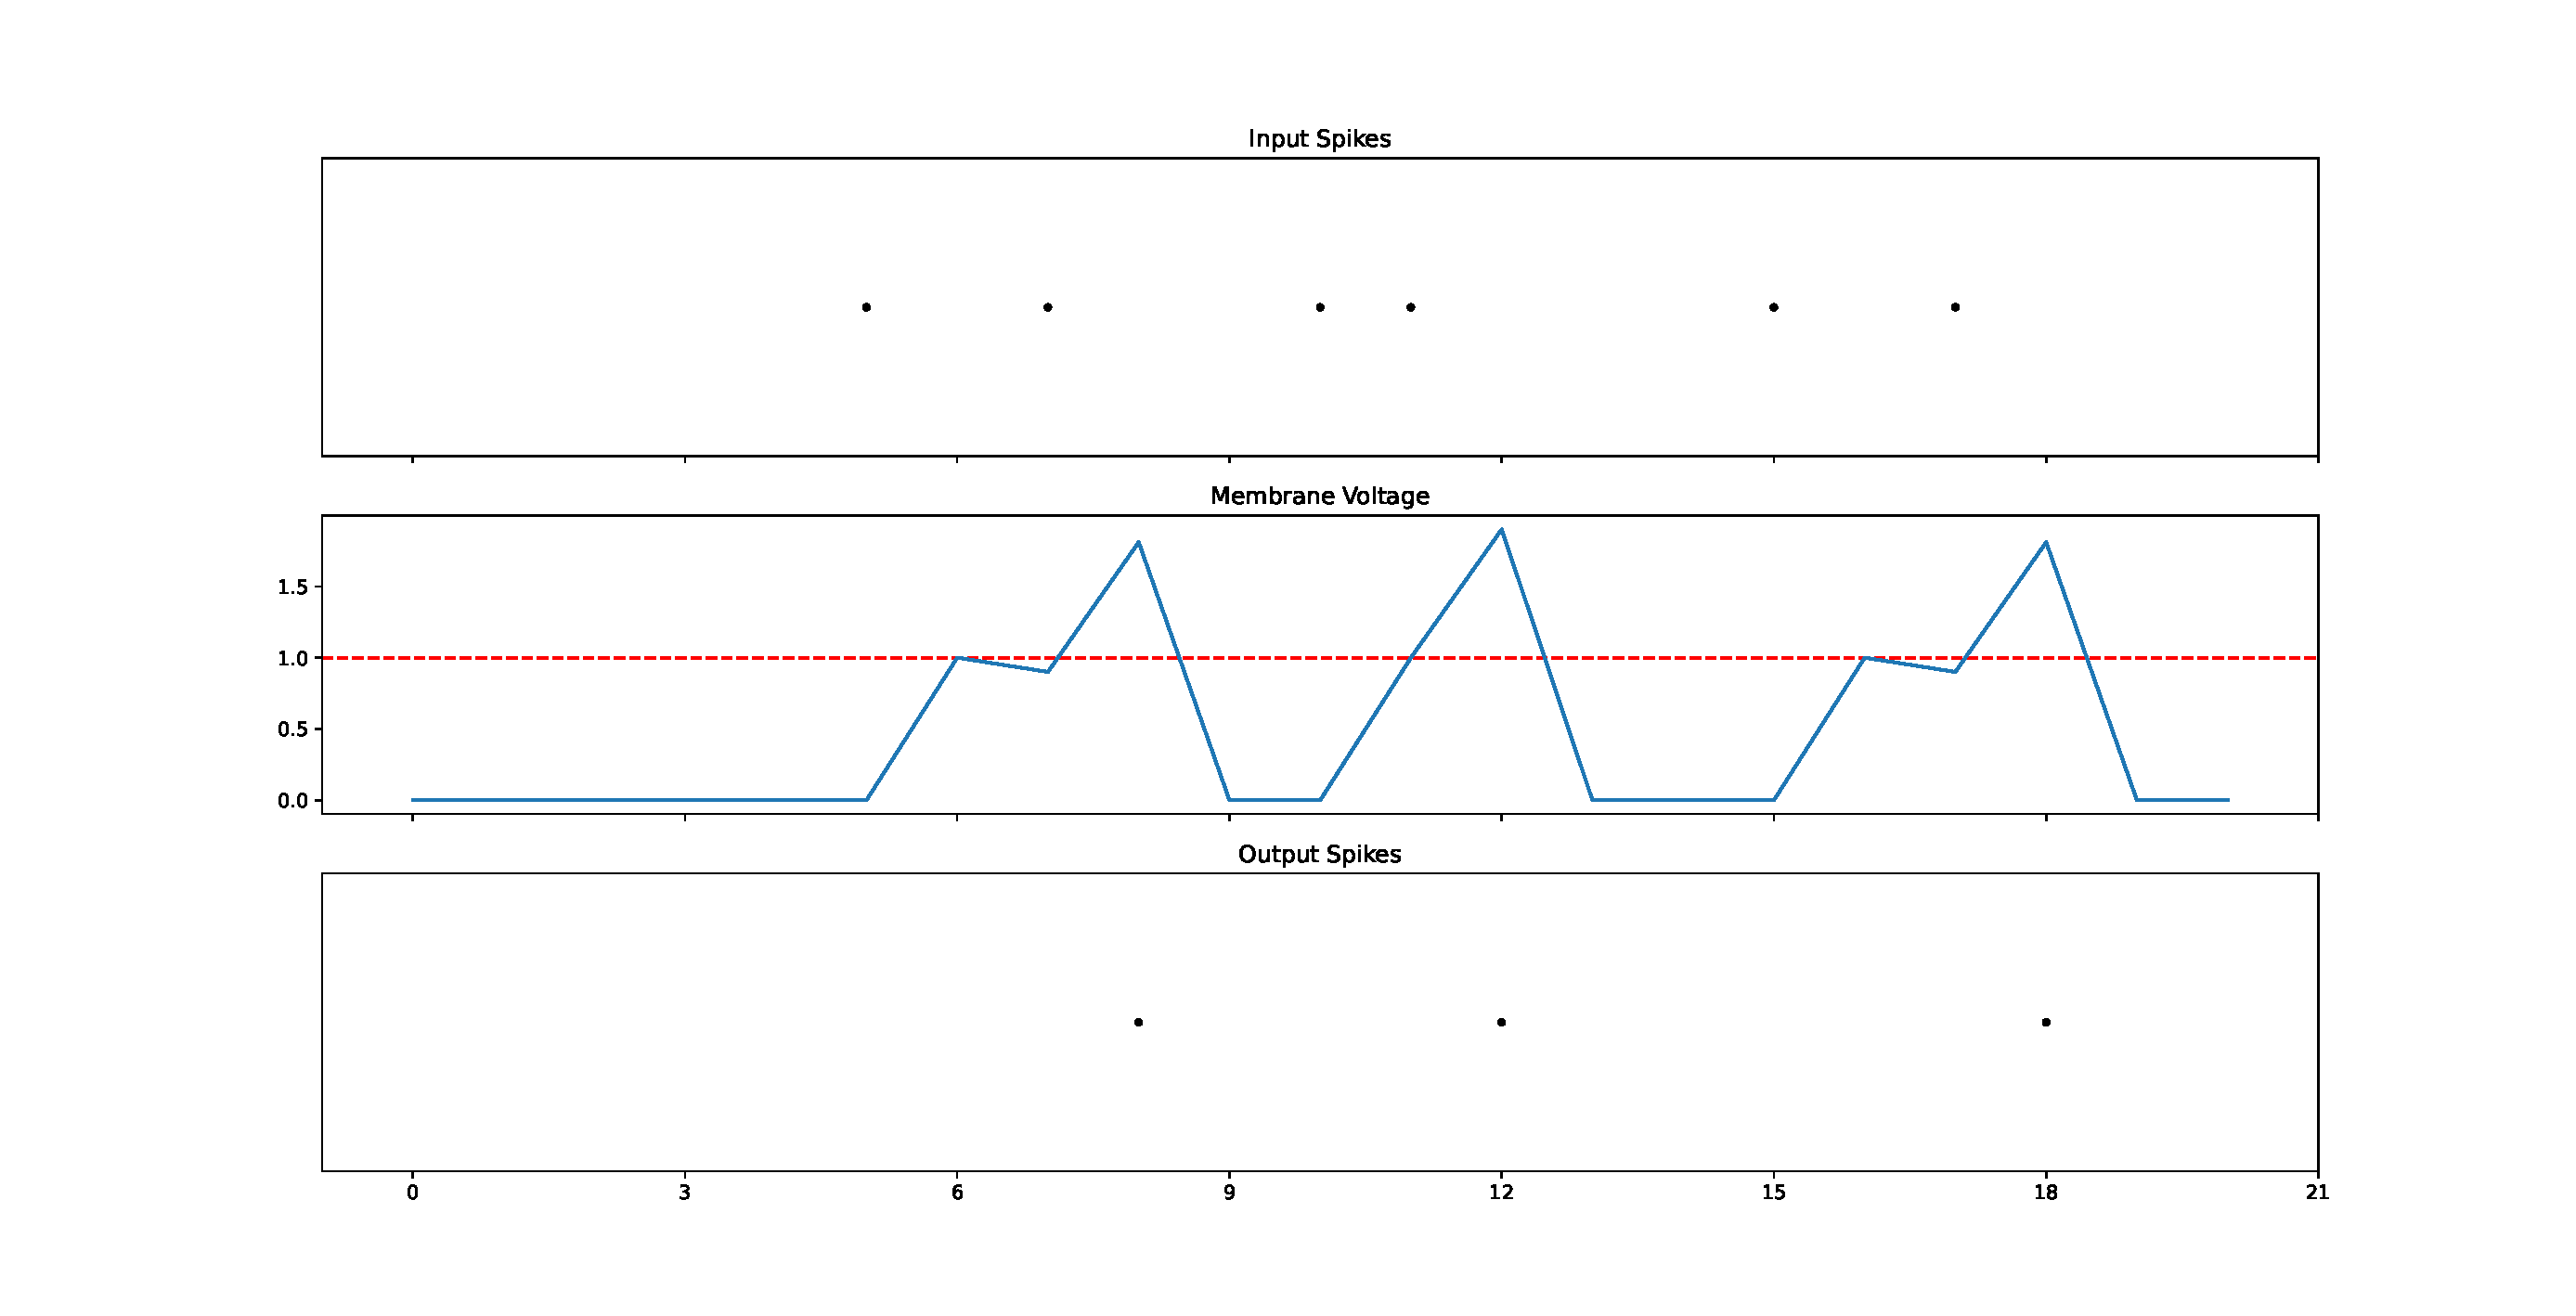
\includegraphics[width=0.7\textwidth]{figures/snn_spike_example.pdf}
    \caption{Demonstrating a LIF neuron. The threshold is represented with the dashed red line.}
    \label{fig:lif_spike_example}
\end{figure}

To summarize, a SNN differs from the classic artificial neural network (ANN) in two fundamental ways. First we replace the activation function with one that only outputs 1's and 0's. Second we have inputs that vary over time. More detailed derivations of SNN theory can be found in Appendix \ref{appendix:snn}.

%********************************************************************%

\subsection{Outputs}

One interesting problem related to SNNs is related to how to interpret the output spike trains. For classification problems, the output layer has one neuron for each possible class. The neuron with the most spikes is chosen as the output label. Our problem, however, is a regression. Thus far, SNN research has focused on classification as there isn't a standard way to interpret spikes into floating point values.

% figure for classification?

To solve this problem, we utilized a linear layer to transform outputs from our SNN into the two angles. One option would be to consolidate the output spike train somehow, such as with a sum or average, and then normalize the values. A technique that hasn't been explored much but was suggested by snnTorch was utilizing the membrane voltages of the last layer. We basically tell the linear layer what each neuron's internal voltage ends at. This also helps with backpropagation, as the network can learn what membrane voltage it should target at the end.

One thing to note is that the network outputs values at each timestep, but we take the result of the last timestep as the guessed values.

%********************************************************************%

\subsection{Architecture}

We base our SNN architecture on that of the LiNet developed by \cite{Masaki}. The LiNet was designed for this task and vastly outperforms fully connected networks. More information about LiNets is provided in appendix \ref{appendix:linet}. To summarize the architecture, it has 5 locally connected layers with one fully connected layer at the end. Each layer has $1/5$ the number of neurons as the previous layer. We simply take the LiNet and replace the ReLU activations with spiking neurons. We keep the fully connected output layer to transform the membrane voltages into our two angles. This model is summarized in \ref{fig:linet_arch}.

\begin{figure}[h]
    \centering
    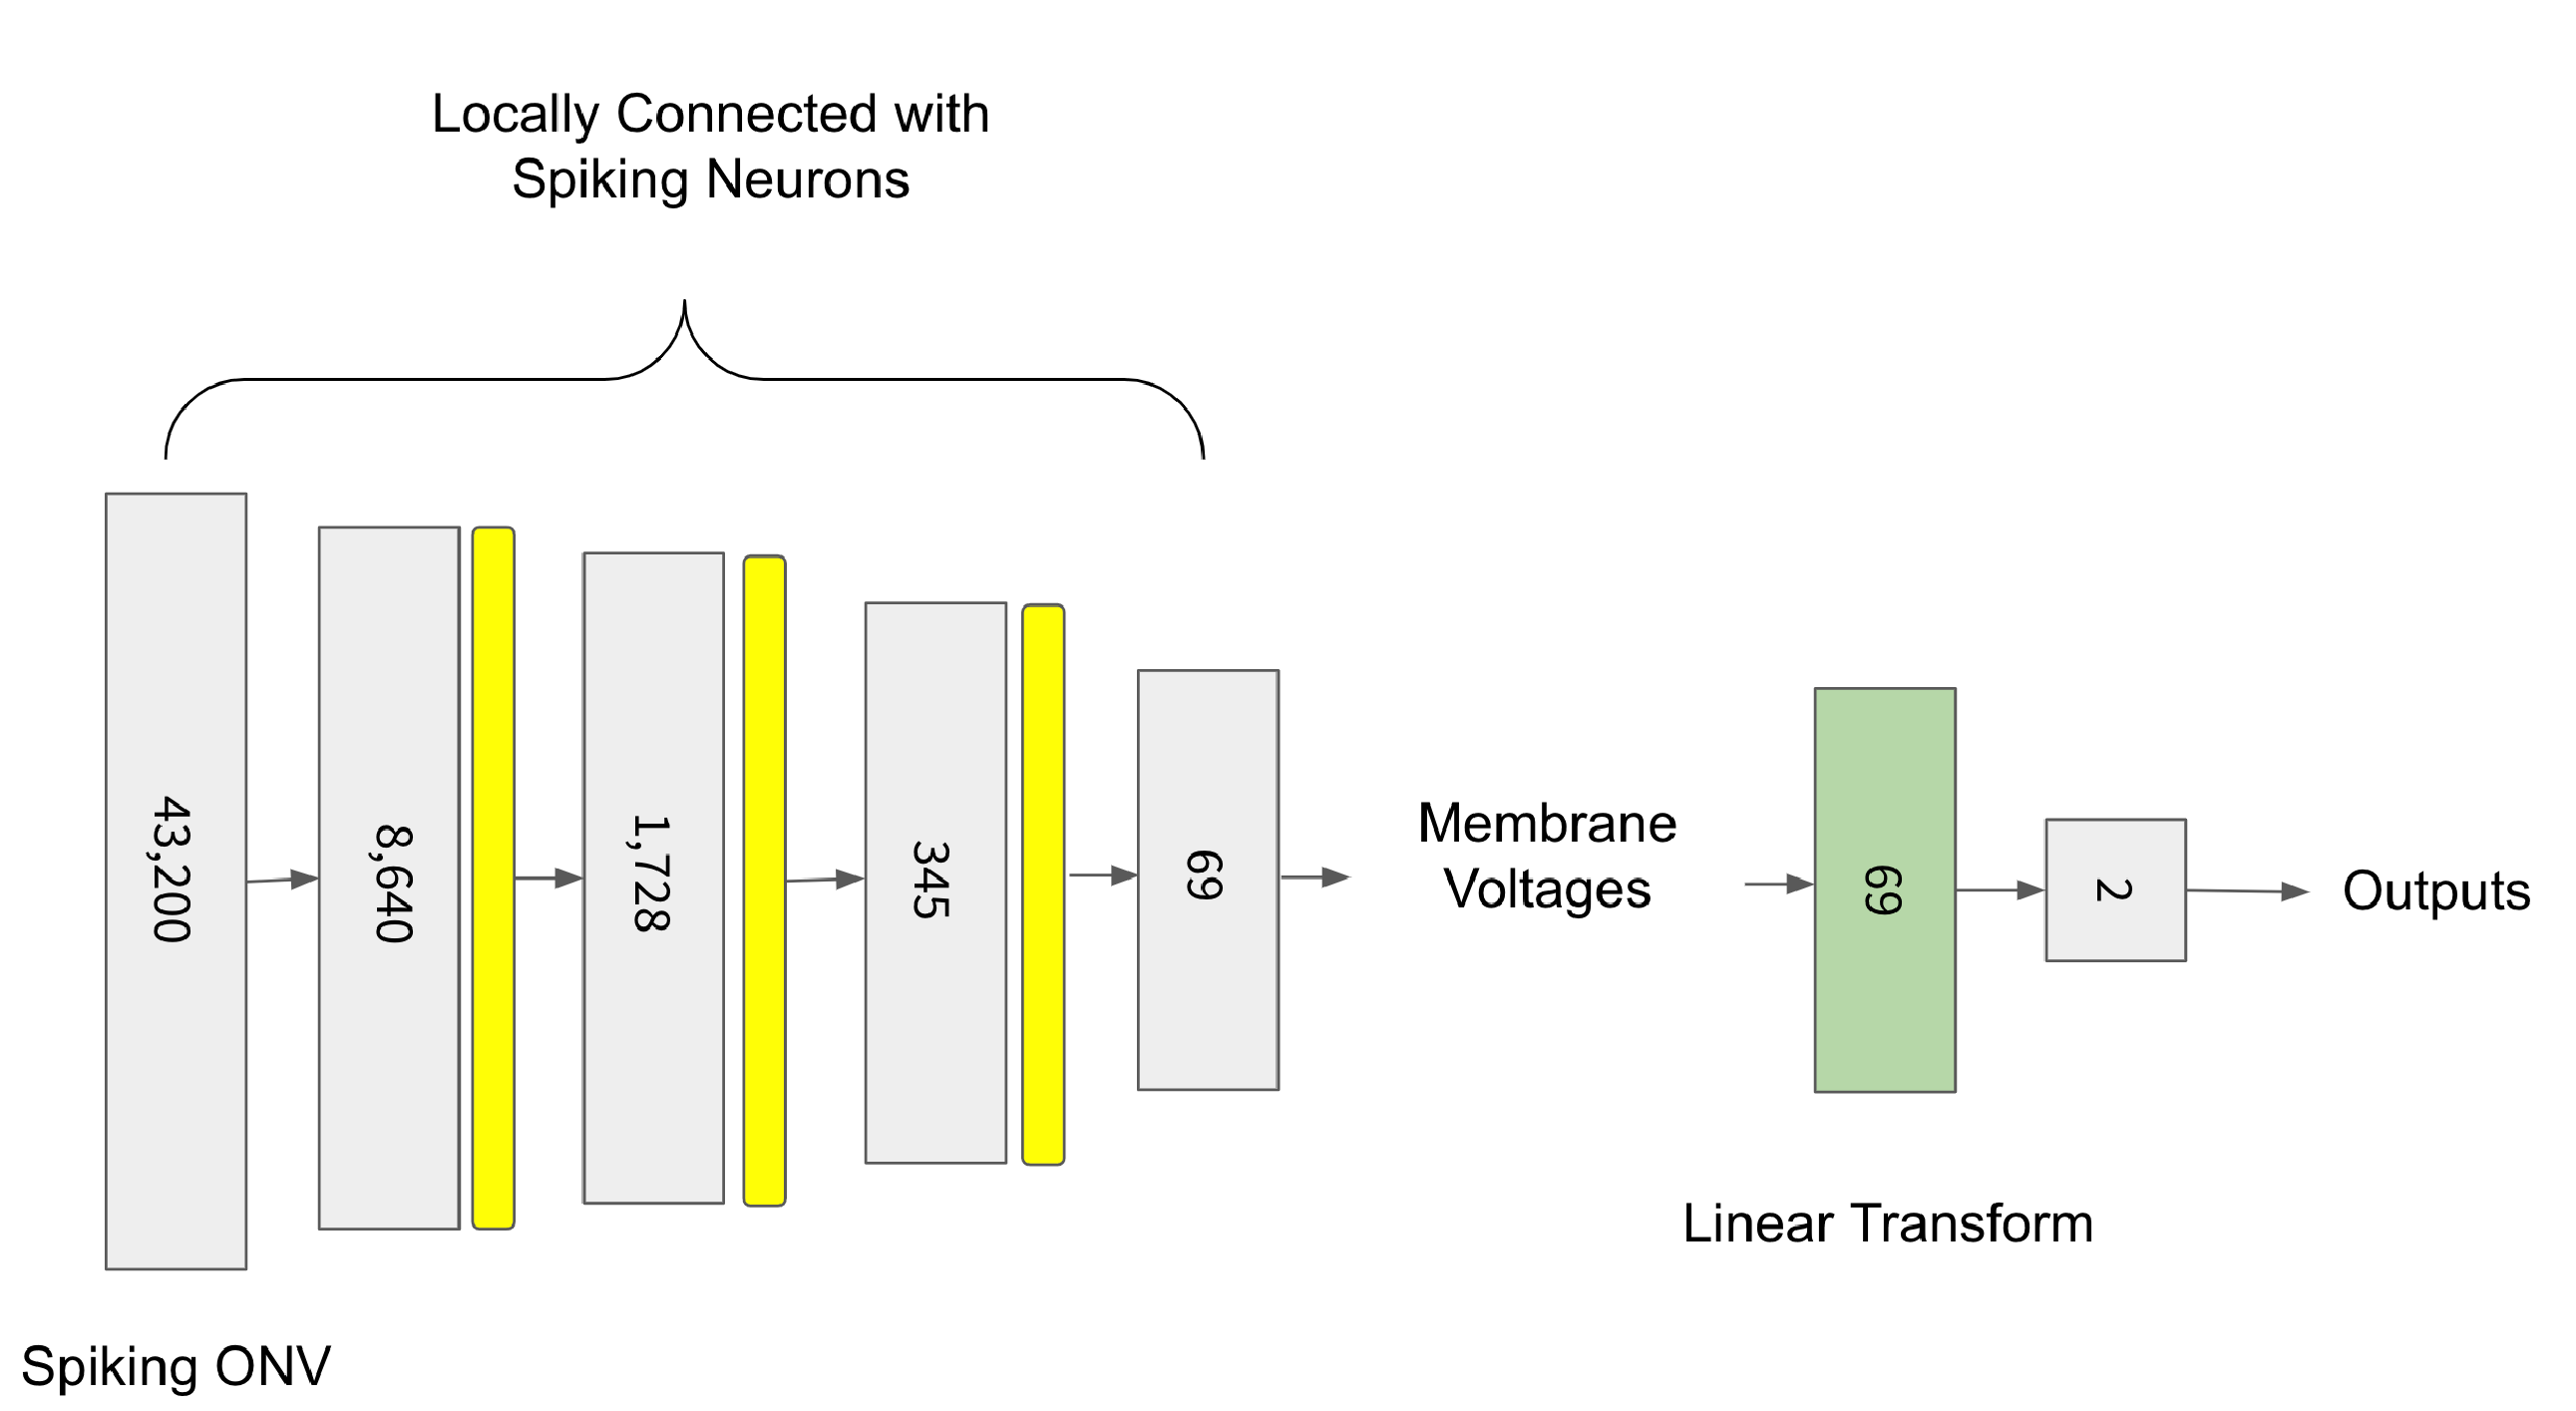
\includegraphics[width=0.7\textwidth]{figures/arch_spiking.pdf}
    \caption{Our spiking LiNet architecture.}
    \label{fig:linet_arch}
\end{figure}

We were also curious to see the effects of adding one spiking layer at a time to a LiNet. We call these models "hybrid SNNs." The architecture has 5 locally connected layers. The first n layers have spiking inputs and the last few use ReLU. There is still one fully connected output layer. The spiking layers compute for a certain number of timesteps and then pass their membrane voltages to the ANN half. This architecture is summarized in figure \ref{fig:hybrid_arch}.

We noticed that adding spiking layers increases noise in the output. With this model, one can make a decision to use a certain number of layers to tradeoff between power usage/latency and accuracy. It also makes computation easier; one can imagine that a neuromorphic chip finishes its work and hands off its result to traditional GPU cores to finish off inference. We only use the more expensive GPU cores for inference on a lower dimensional vector.

\begin{figure}[h]
    \centering
    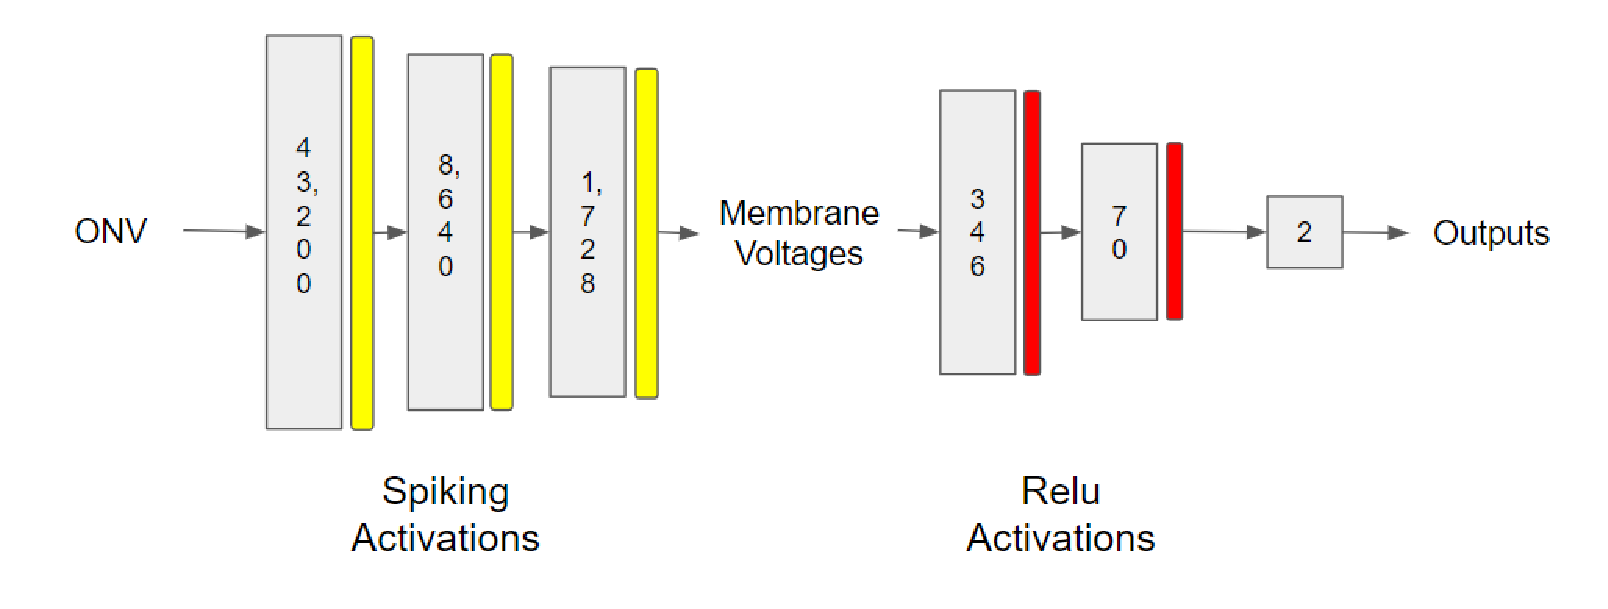
\includegraphics[width=0.7\textwidth]{figures/arch_hybrid.pdf}
    \caption{Our Hybrid Spiking LiNet architecture.}
    \label{fig:hybrid_arch}
\end{figure}

% code comparison between ANN, SNN, and Hybrid
% TODO: labels, refer above
\noindent\begin{minipage}{.45\textwidth}
\lstinputlisting[language=Python, firstline=1, lastline=12, caption=Normal feedforward network.]{figures/code1.py}
\end{minipage}\hfill
\begin{minipage}{.45\textwidth}
\lstinputlisting[language=Python, firstline=15, lastline=35, caption=SNN feedforward network with spiking activation functions and an input that varies over time.]{figures/code1.py}
\end{minipage}

\lstinputlisting[language=Python, firstline=37, lastline=59, caption=A hybrid SNN that hands off its output to an ANN]{figures/code1.py}

%********************************************************************%

\subsection{Training}

Here we go over the various decisions made while training our SNNs.

By default, all neuron thresholds are set to one. These can optionally be trained as part of backpropagation; we found that a random initialization converged better than initializing them to one.

When a neuron outputs a spike, there are two options related to how to reset the membrane voltage. One is called "zero" because the voltage is simply set to zero. The other, called "subtraction", subtract the threshold value instead. This allows the neuron to have a non-zero membrane voltage at the next timestep, where the reset happens. We empirically found that subtraction performs better than reset.

\subsubsection{Number of Steps}

The number of timesteps to run the SNN for is a hyperparameter. More time steps allow more neurons to fire downstream, which may help computation but will also require more energy to run. Conversely, models using a lower number of timesteps may train quickly but have difficulty converging to a low enough loss value. Typical values are in the hundreds or thousands. After doing a hyperparameter sweep we empiriaclly found that 20 timesteps was enough for the model to converge. Higher numbers of steps were more difficult to train and didn't seem to affect performance.

% this is odd, have graphs of loss for various timesteps?


\subsubsection{Surrogate Gradients}

On the backpropagation pass, we encounter the heaviside step function as our spiking activation function. Its local derivative is 0 everywhere except for the time of the spike, where it is infinite. This is the main barrier to deep learning with spiking neural networks as our gradient will either become 0 or infinity. snnTorch handles this by passing through the gradient when there is a spike and 0 when there isn’t. This enables some learning, but is not good enough for this task. The library also implemented surrogate gradients, which are functions that approximate the heaviside step function but are differentiable everywhere. The spiking activation is still used in the forward pass, but we use the surrogate gradient on the backward one. This approximation yields good results.

% math of backprop with step func?

The approximation used is the fast sigmoid function, named as it is faster to compute than the normal sigmoid function.

% figure of sigmoid and its derivative
\begin{figure}[h]
    \centering
    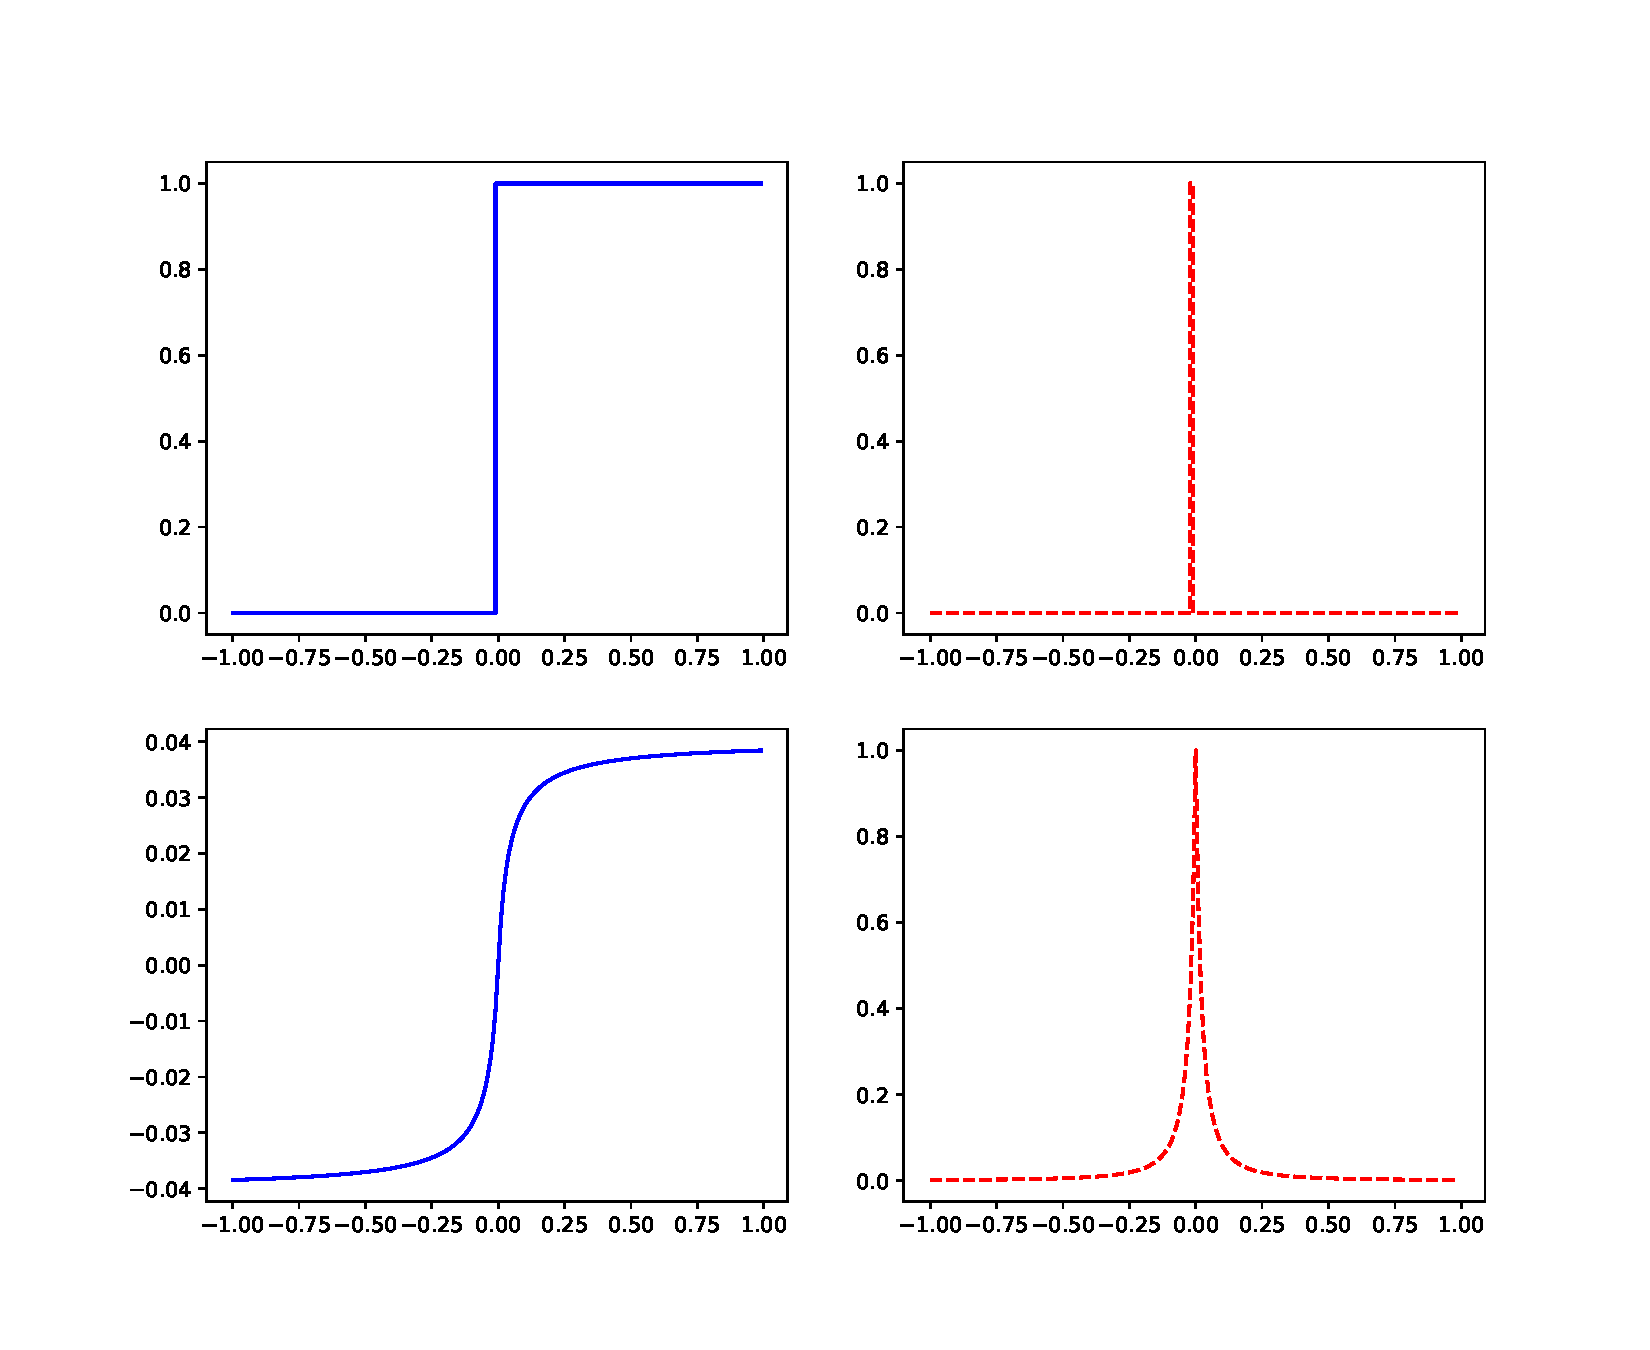
\includegraphics[width=0.7\textwidth]{figures/surrogate_grad.pdf}
    \caption{We compare the derivative of the heaviside step function and that of the fast-sigmoid function.}
    \label{fig:surrogate_grad}
\end{figure}

\subsubsection{Loss Calculation}

The SNN computation graph can be unrolled exactly like a recurrent neural network (RNN), so backpropagation through time (BPTT) is used. One trick can be employed to encourage the SNN to reach correct outputs faster. This involves collecting the output from each timestep, calculating the loss with the expected value, then summing all of these losses together. This unfortunately required more memory than our GPU could handle, so we could not experiment with this method.

%********************************************************************%

\subsection{Convert ANN}

The ideas from this section are relevant only if one is training an SNN from scratch like we do. If one does not want to do this, there exist methods to convert an existing, trained ANN into a SNN. Converting an ANN allows one to not deal with the non-differentiability of the spiking activation function. The main drawback of this method is that it requires a large number of timesteps to run, usually on the order of thousands. Furthermore, one of the goals of this thesis was to work with event-based data, and the spike encoding methods to work with a converted SNN are not biologically inspired.

One class of methods does not allow for models with biases in each layer. We attempted to train a LiNet without biases but it could not converge, so we ruled these methods out.

More recent papers have shown how one can convert complex layers such as convolution layers and also use biases. This involves scaling the weights layer by layer. Inspired by \cite{rathi2020enabling}, we tried an approach where we first scaled the weights and biases as an initialization step. We then trained this model on the data using the fast sigmoid surrogate gradient. The model had trouble converging so we do not report comparisons between training an SNN from scratch vs converting an ANN.


%%%%%%%%%%%%%%%%%%%%%%%%%%%%%%%%%%%%%%%%%%%%%%%%%%%%%%%%%%%%%%%%%%%%%%

\end{document}